\documentclass{standalone}
\usepackage{pgfplots}
\usepackage{amsmath}
\usepackage{textcomp}
\pgfplotsset{compat=1.18}

\begin{document}

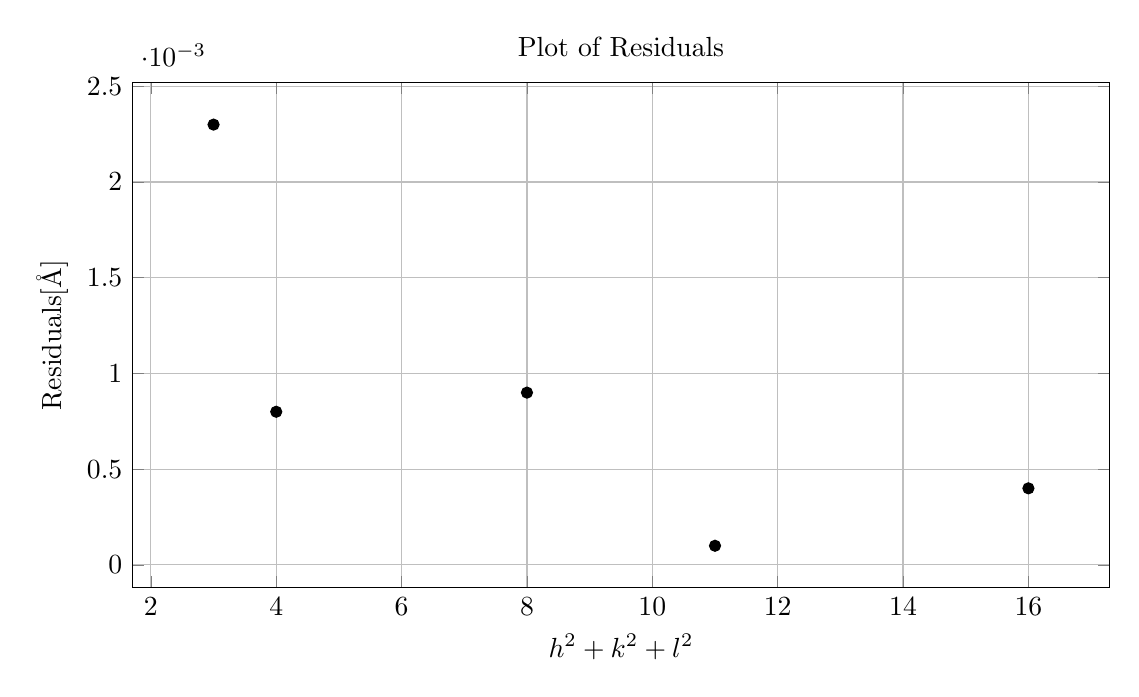
\begin{tikzpicture}
\begin{axis}[
    xlabel={$h^2 + k^2 + l^2$},
    ylabel={Residuals[\AA]},
    title={Plot of Residuals},
    grid=both,
    width=14cm,
    height=8cm,
    legend style={at={(0.015,0.96)}, anchor=north west}
]

% 実験データ点
\addplot[
    only marks,
    mark=*,
    color=black,
]
coordinates {
  (3,0.0023)
  (4,0.0008)
  (8,0.0009)
  (11,0.00010)
  (16,0.0004)
};
\end{axis}
\end{tikzpicture}

\end{document}
